%!TEX root = ../report.tex

\chapter{Natural Language Processing}

Natural Language Processing evolved as a branch of artificial intelligence by combining fields such as computer science and linguistics. It helps machines to comprehend, manipulate and generate human language. Natural language processing gained interest as it seemed promising in various tasks such as human-machine interaction / communication, machine translation, spam detection, voice controlled devices, summarizing texts, and question answering in search engines \cite{nlp_appli}. Thanks to the availability of a large number of unstructured data that is created everyday (for eg. social media and medical records), efficient algorithms and powerful computing systems, a lot of advancements have been made in this field in the last few decades. 

Though natural language processing is an exciting field which enables everyone to communicate with the computers in their own language (as opposed to the programming language or low level language used by the computer), understanding and making sense of human language has many layers of difficulty. The complex and diverse nature of human language, unique sets of rules and grammars for different languages, new meaning of words, different meanings for the same word, and abbreviations restrict the ability of computers to make sense of natural language. Though humans are capable of expressing, perceiving, and interpreting very elaborate and nuanced meanings, they still lack at formally defining the rules that govern the language \cite{goldberg2017neural}. This hinders the capability of taking a rule-based approach towards natural language understanding by computers as rules differ for every language and word ambiguations is commonplace. 

Many Natural Language Processing tools and methods are used to bring the natural language into a format which could be made sense by computers. These techniques enable computational methods to manipulate data and make inferences from them such as how similar two sentences are, whether one sentence could be infered from another sentence, and determining the topic of an article. The most prominent NLP methods and tools are discussed below. 

\section{Pre-processing methods in NLP}

Pre-processing the text helps in bringing the input data into a form which could be digested by the algorithm. While such methods would help in computational methods, it is important to note that some of the details could be lost from the original input and the key idea is to know the pros and cons of each of these methods and to apply them where necessary.

\subsection{Tokenization}

Tokenizations is a process of text segmentation which helps in splitting the text into sentences or sentences into words. Such sentences or words are called as 'tokens'. Common ways of doing this include splitting on whitespaces and splitting on punctuations. However, splitting a sentence based on whitespace or punctuations is not a straightforward task as complex words need careful attention while splitting them; e.g. "Los Angeles", "Mr. Mercedes", "i.e.", "Simon's cat", "on-campus housing" etc. To deal with such cases, rule-based or machine learning approached could be applied \cite{jurafsky2014speech}.

\subsection{Normalization}

This method is utilized to bring all text into the same format so that manipulating them would be less biased and uniform across different forms of sentences and phrases. Simple tasks such as removing punctuations, converting numbers into their word forms, and converting all text to lowercase help in putting all the data on equal footing. Though these methods sound easy, attention must be given to minute details; e.g. converting "US" to "us" does not give the same meaning. Normalization in NLP is equivalent to normalizing all the image pixels in a computer vision task so that the algorithm doesn't give importance to more colorful or vibrant images. Other normalizing methods that are used in this report includes stemming and lemmatization. 

\subsection{Stop words removal} 

Stop words should be filtered out before processing the text further as they occur more frequently in text and contribute little to the overall meaning of it while serving the purpose of connecting different parts of a sentence. Some of the most common stop words in English include "the", "so", "and", "it", and "a" \cite{nltk_list}. As can be seen from the following example, stop word removal does not change the overall meaning much. 

\vspace{2mm}

input = "The player hits the ball over the fence"

output = "player hits ball over fence"

\subsection{Stemming and Lemmatization}

These words convert the words into their base or common form. Stemming does this by dropping unnecessary characters, suffixes, prefixes, infixes, and circumfixes from a word in order to obtain a word stem \cite{kdnuggets_preprocessing}. The results of stemming could be used to find relationships and similarities between large text documents. An example of stemming could be seen as follows.

\vspace{2mm}

input = "I started studying yesterday"

output = "I start studi yesterday"

Lemmatization converts the words to the base form after going through the vocabulary and doing a morphological analysis like part-of-speech of every word \cite{jurafsky2014speech}. Lemmatization can produce better results by utilizing WordNet's lexical database of English. It offers more accuracy at the cost of time as it is an intensive and slower process. Stemming is more useful where simple database queries are carried out and time is an important factor, while lemmatization could be used for more complex tasks such as sentiment analysis.

\section{Word Embedding}

Word embedding is a NLP task which converts text into an array of numbers or real valued vectors. Such a representation of words proved to be useful in many tasks such as semantic similarity measures, text classification, and machine translation. Though one-hot-encoding (where a sentence is represented by a matrix with its dimension equal to the number of words in the sentence and each row made up of 0's with a 1 in the dimension corresponding to the word) was used in the beginning as a word embedding model, it has issues such as being a sparse matrix, redundant memory, and inability to capture the context or the relationship between different words in the same sentence. 

More compact and meaningful representations of words evolved later with the use of neural networks and a large corpora to learn the distributions of words on. The most popular algorithms which exist today for efficient word embedding include Google's Word2Vec \cite{word2vec}, Facebook's fasttext \cite{fasttext}, and Stanford's GloVe \cite{glove}. These algorithms were able to capture both the semantic relationships and context of each word and represent them in a more compact way (dense vectors) \cite{shane_wordembedding}. Fig \ref{simple_embedding} below depicts a 2D representation of word embeddings where similar words in context and meaning have been grouped together in the vector space. 

\begin{figure}[h!]
	\centering
	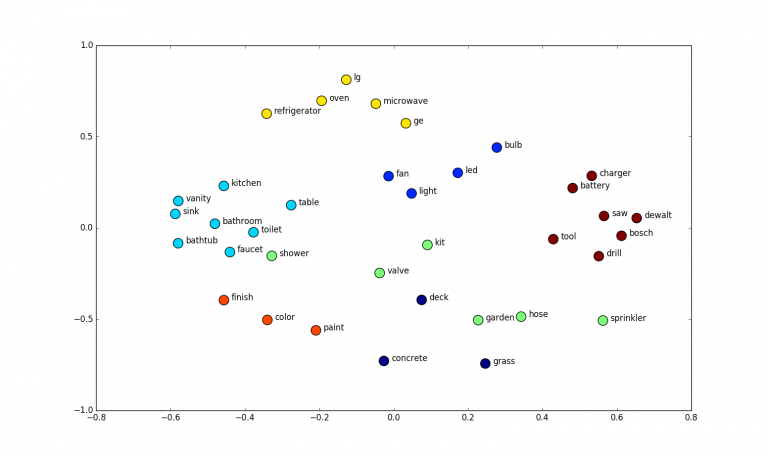
\includegraphics[scale=0.5]{images/2d_word_embedding}
	\caption{Example 2D word embedding space, where similar words are found in similar locations. \cite{2d_embedding}.}
	\label{simple_embedding}
\end{figure}

\section{Libraries and Toolkits}

In order to do seamless experiments, a lot of libraries and toolkits came in handy while parsing, preprocessing the text, and extracting the features. These libraries include functions which would do the most repititive tasks in NLP that would require a significant time to code from scratch. The open source libraries which were used in our experiments include Numpy, Pandas, NLTK, Spacy, and scikit-learn. These will be discussed below.

\subsubsection{Numpy}

Numpy is a very useful library in Python which could be used to work with multidimensional arrays and matrices along with some high-level mathematical functions to operate on these arrays. In addition, it has functions with linear algebra, Fourier transform, and random number capabilities \cite{numpy}.

\subsection{Pandas}

Pandas provides high-end, easy-to-use datastructure and data analysis tools written in Python programming language \cite{pandas}. It was helpful in filtering out the required fields from the dataset and visualize the results of preprocessing steps in a structured manner.  

\subsection{NLTK - Natural Language Toolkit}

Natural Language Toolkit is a platform for working on human language using Python. It is open-source and one of the most versatile libraries available today. It has a easy-to-use interface to over 50 corpora and lexical resources such as WordNet. In addition, it has functionalities for various NLP tasks including  classification, tokenization, stemming, tagging, parsing, and semantic reasoning \cite{nltk}.

\subsection{spaCy}

spaCy is a free open-source library for Natural Language Processing, written in the programming languages Python and Cython. It is more suitable for large-scale information extraction tasks as it is fast and efficient. With seamless interoperation with most of the deep learning libraries and frameworks. Non-destructive tokenization, Named entity recognition, Support for 31+ languages, 13 statistical models for 8 languages, Pre-trained word vectors, and Part-of-speech tagging are some of its features. Opposed to NLTK, which is widely used for teaching and research, spaCy is focused more on providing software for production usage \cite{spacy}.

\subsection{scikit-learn}

scikit-learn is a simple and efficient tool for data mining and data analysis which is built on top of Numpy, Scypy and matplotlib. It is a open-source library written in Python programming language. The most prominent algorithms built in this library include classification, regression, clustering, dimensionality reduction, model selection and preprocessing. We used scikit-learn to employ different machine learning algorithms which would suit best for out task such as logistic regression and support vector machines (SVMs) \cite{scikit_learn}. 